\documentclass[11pt]{article}
\usepackage{amsmath, amssymb, amscd, amsthm, amsfonts}
\usepackage{graphicx}
\usepackage{tikz}
\usepackage[]{tikz-3dplot}
\usepackage[colorlinks]{hyperref}
\usepackage[nameinlink,noabbrev]{cleveref}
\usepackage{float}
\usepackage[labelfont=bf]{caption}
\usepackage{subcaption}
\usepackage[a4paper, total={6in, 8in}]{geometry}
\usepackage{soul}
\usepackage{enumitem}   

%\oddsidemargin 40pt
%\evensidemargin 40pt
%\marginparwidth 40pt
%\marginparsep 40pt
\topmargin 0pt
\headsep 0pt
\textheight 8.7in
%\textwidth 6in
\linespread{1.2}

\title{Deep Learning FSS22 \\ Assignment 3: Hyperparameter Optimization}
\author{Timur Michael Carstensen - 1722194}
\date{05.06.2022}


\newcommand{\rr}{\mathbb{R}}

\DeclareMathOperator*{\argmax}{arg\,max}
\DeclareMathOperator*{\argmin}{arg\,min}

\newcommand{\al}{\alpha}
\DeclareMathOperator{\conv}{conv}
\DeclareMathOperator{\aff}{aff}

\begin{document}

\pagenumbering{roman}

\maketitle


\newpage

\tableofcontents

\newpage


\pagenumbering{arabic}

\section{Basic Hyperparameter Tuning}\label{sec:cnn}

\subsection{a)}\label{subsec:basic-a}

The results for the manual hyperparameter search can be seen in \autoref{fig:1a}. We first tried to get an overview of the hyperparameter space by exploring evenly in the first nine trials. That is, we tried all combinations of $x_1\in\{0, 0.5, 1\}$ and $x_2\in\{0, 0.5, 1\}$. Then, we observed that lower function values were seen in the top-right quadrant of the hyperparameter space and focussed our search on that area. After observing that the function values increased around $[0.7, 1]$, we evaluated the function more in the middle of the top-right quadrant and achieved a function value of $-3.0$ with $[0.7, 0.7]$. Finally, we tried to evaluate $f_1$ at $[0.8, 0.8]$ and achieved a function value of $-7.83$. Given that the function value decreased so quickly for such a small difference in function inputs, we can conjecture that the validation loss surface is not well-behaved and that there are many local optima to this function. Therefore, we believe that we found a good result. 


\begin{figure}[H]
  	\center
  	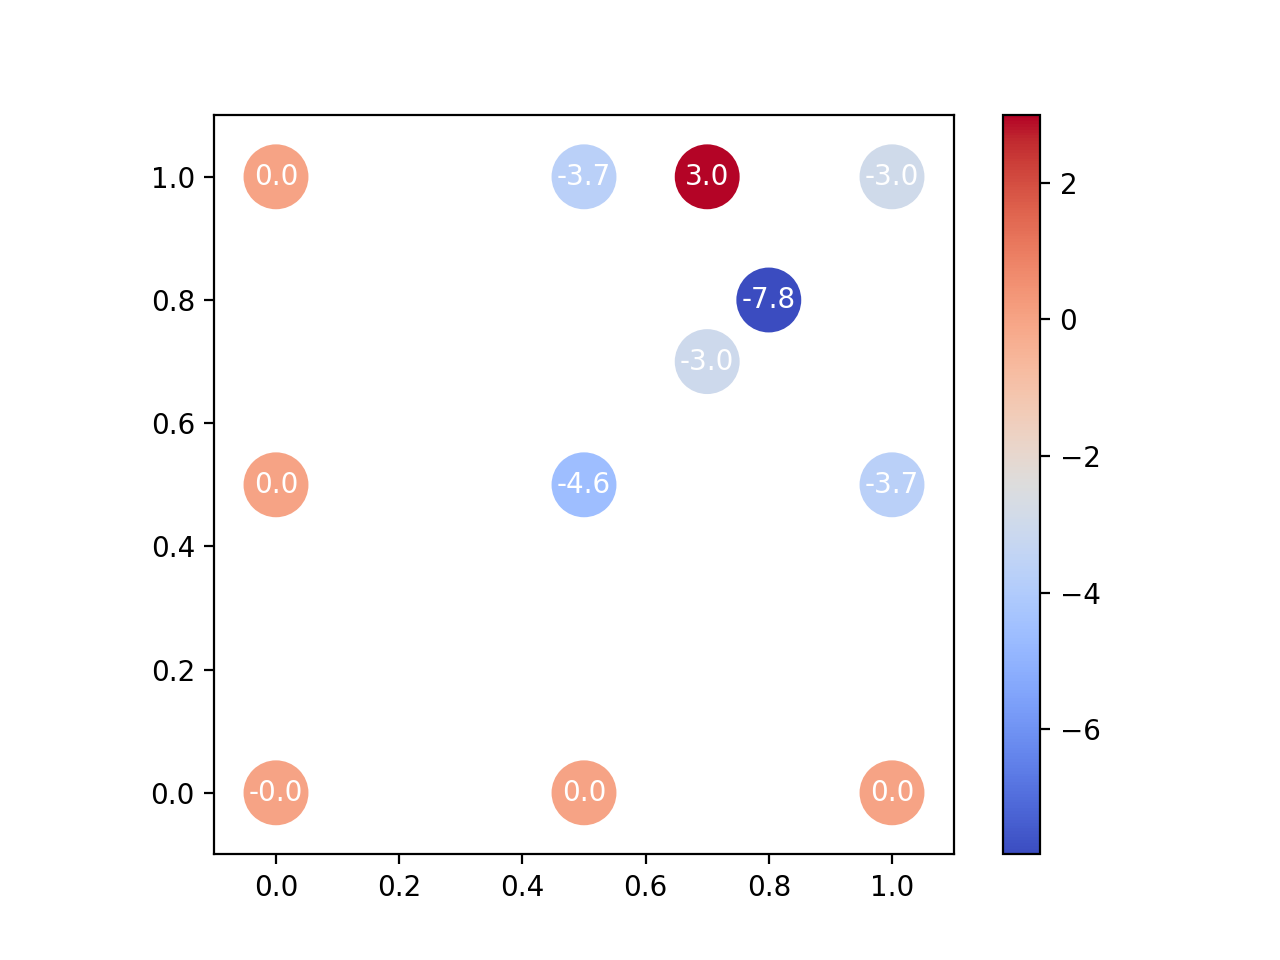
\includegraphics[width=.6\columnwidth]{assets/1a}
  	\caption{Results obtained for the manual hyperparameter search.}
  	\label{fig:1a}
\end{figure}


\subsection{b)}\label{subsec:basic-b}

The plot of $f_1$ shown in \autoref{fig:1b} confirms our belief from \autoref{subsec:basic-a}. We found a function value of $-7.83$ with $[0.8, 0.8]$ while the true global minimum of the function is $-7.88$ with $[0.7917, 0.7917]$. That is, we got extremly close to the global minimum within the 12 trials that we performed. The plot also shows that the surface of $f_1$ is not well-behaved as it has many (4) local minima. That is the surface has many peaks and valleys and is not convex. 

\begin{figure}[H]
	\centering
	\begin{subfigure}[b]{0.47\textwidth}
		\centering
		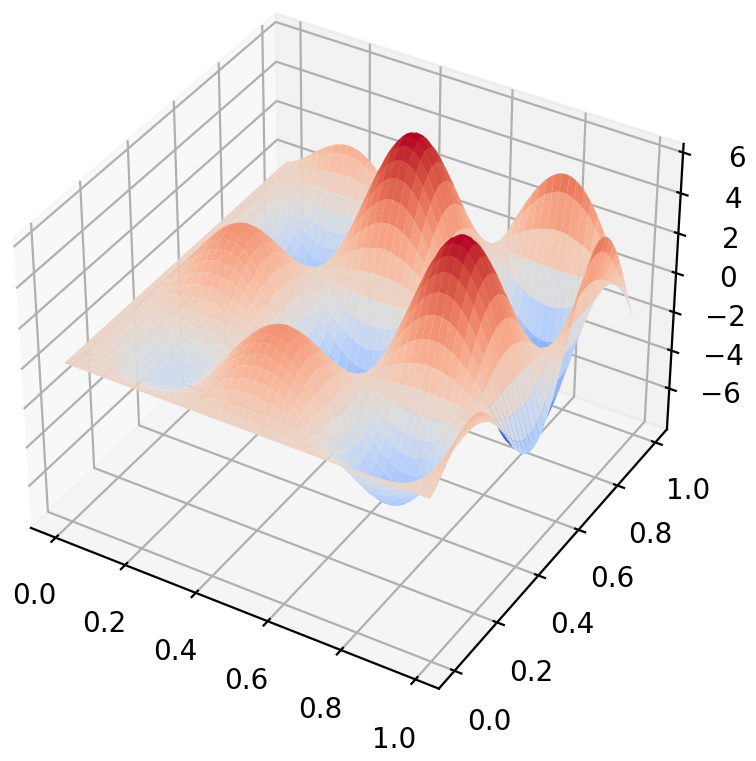
\includegraphics[width=\textwidth]{assets/1b-3d}
		\caption{}
	\end{subfigure}
	\begin{subfigure}[b]{0.47\textwidth}
		\centering
		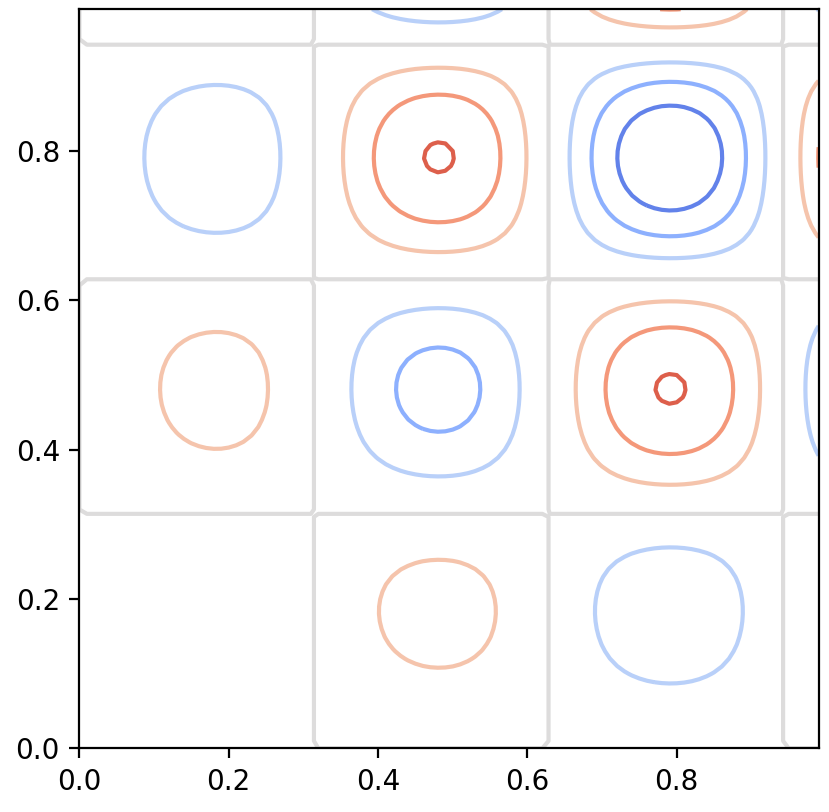
\includegraphics[width=\textwidth]{assets/1b-contour}
		\caption{}
	\end{subfigure}
	\caption{Function surface of $f_1$; (a) 3D plot, (b) contour plot}
	\label{fig:1b}
\end{figure}

\subsection{c)}\label{subsec:basic-c}

The results of the grid search can be seen in \autoref{fig:1c}. We split the two hyperparameters ($x_1, x_2$) into 3 and 4 equidistant points ($x_1\in\{0, 0.5, 1\}$ and $x_2\in\{0, \frac{1}{3}, \frac{2}{3}, 1\}$) and evaluated $f_1$ for all possible combinations of the two paramters. The grid search method did not find the global minimum, which is to be expected given the knowledge about it's location. This is coherent with what we learned in the lecture. That is, grid search only explores $n^{1/L}$ values per hyperparameter for $n$ trials and $L$ hyperparameters. In our case: $L=2, n=12 \text{ and } 12^{1/2}=3,46$ which is very close to the average of the parameters that we did explore: $\frac{4+3}{2}=3.5$. 

\begin{figure}[H]
  	\center
  	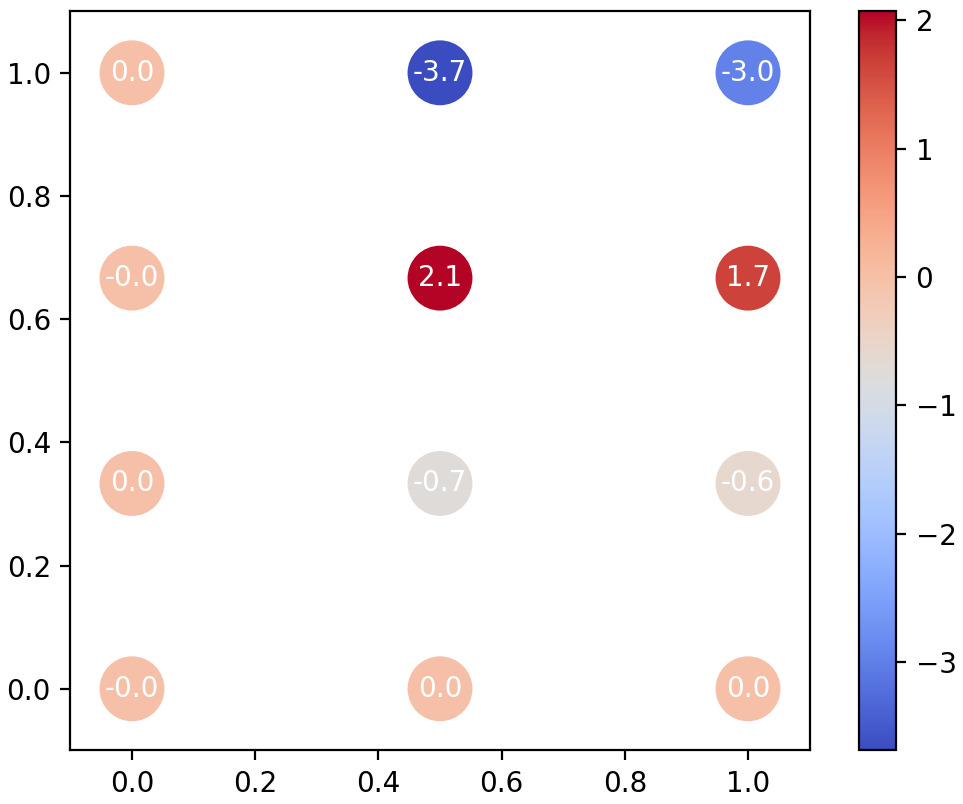
\includegraphics[width=.5\columnwidth]{assets/1c}
  	\caption{Results obtained for the manual hyperparameter search.}
  	\label{fig:1c}
\end{figure}

\subsection{d)}\label{subsec:basic-d}

The results of multiple runs of random search are shown in \autoref{fig:1d-random}. We can see that a lot of the hyperparameter configurations are "clustered" together. That is, there are many redundant trials. For example, in \autoref{fig:1d-random} (a) we can observe that the hyperparameter space is not explored in the top-left quadrant (not at all, actually). Conversely, the range of hyperparameter configurations between $x_1 \in [0.5, 0.65]$ and $x_2 \in [0.2, 0.4]$ are explored with four trials. A similar clustering of evaluated hyperparameter configurations can be see in \autoref{fig:1d-random} (c). Out of the three runs that we performed, only the one in \autoref{fig:1d-random} (b) achieves a somewhat good exploration of the hyperparameter space, given the prespecified budget.\\

\begin{figure}[H]
	\centering
	\begin{subfigure}[b]{0.325\textwidth}
		\centering
		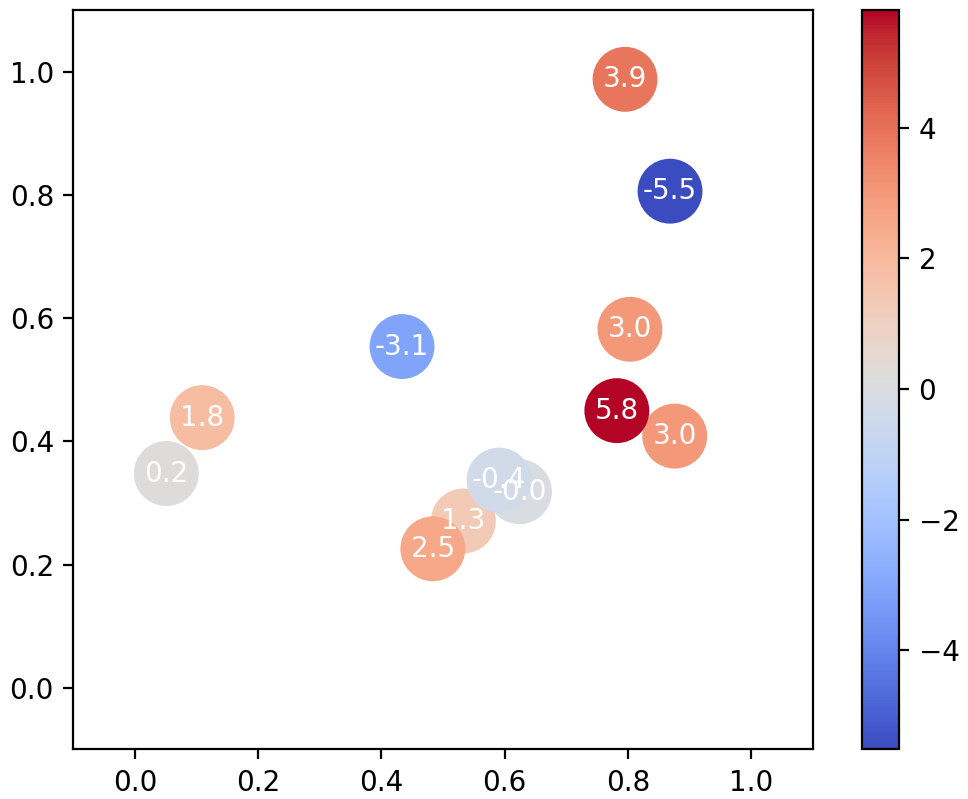
\includegraphics[width=\textwidth]{assets/1d-1st}
		\caption{}
	\end{subfigure}
	\begin{subfigure}[b]{0.325\textwidth}
		\centering
		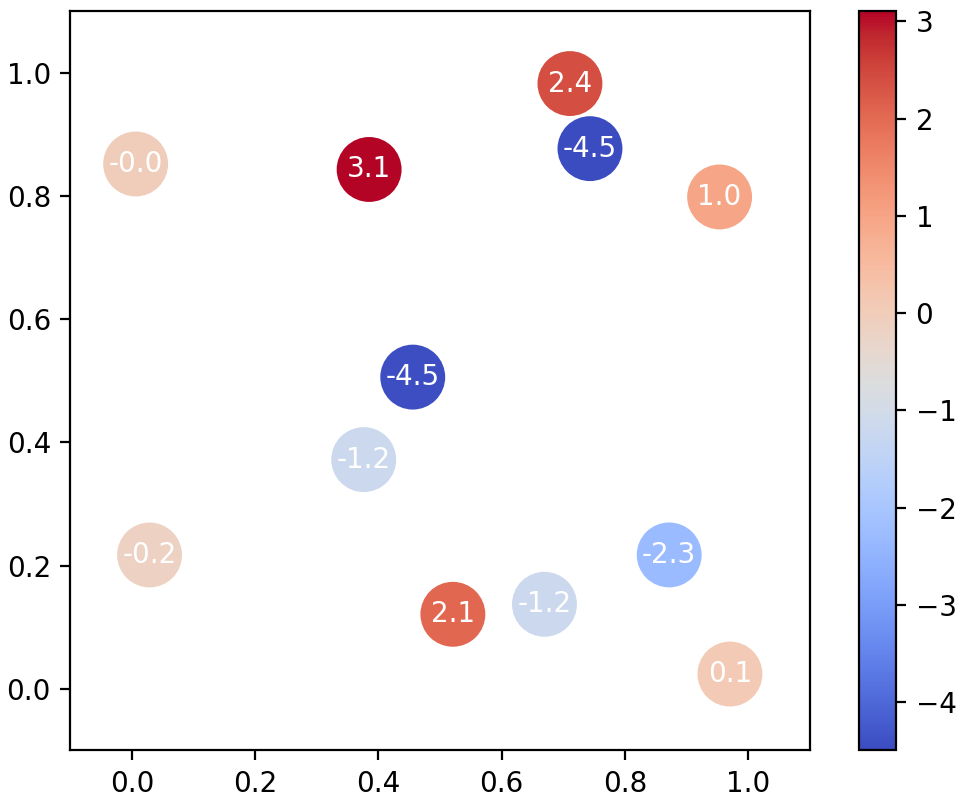
\includegraphics[width=\textwidth]{assets/1d-2nd}
		\caption{}
	\end{subfigure}
	\begin{subfigure}[b]{0.325\textwidth}
		\centering
		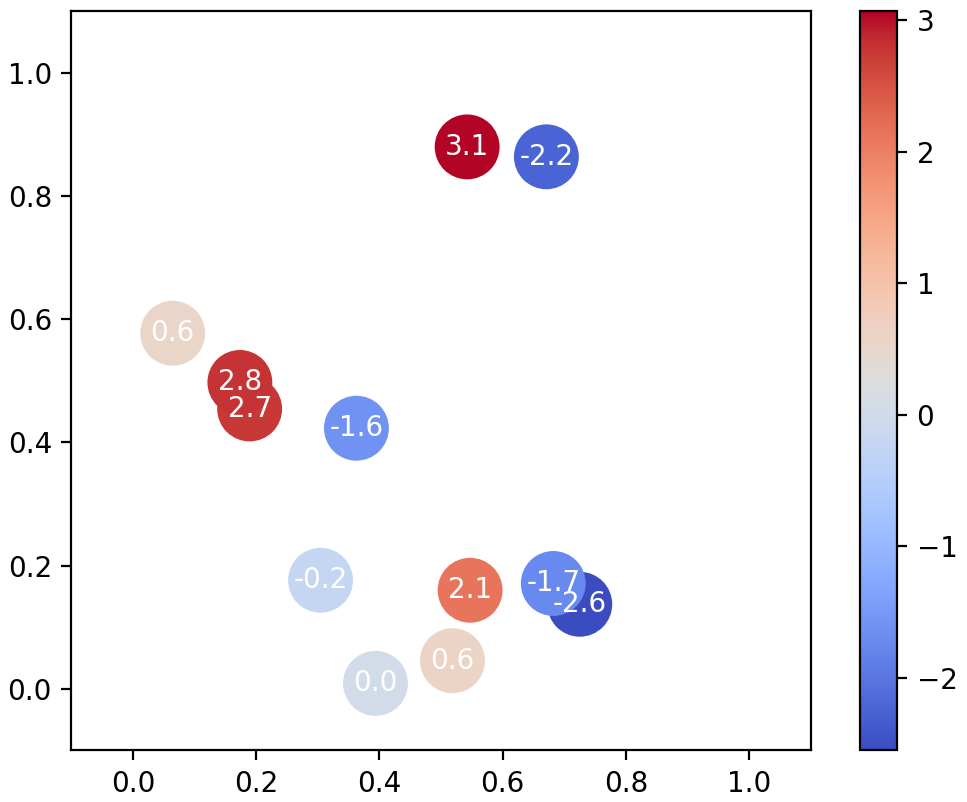
\includegraphics[width=\textwidth]{assets/1d-3rd}
		\caption{}
	\end{subfigure}

	\caption{Results of three random search trials using random uniform sampling for the hyperparameters for $f_1$ shown in (a), (b), and (c).}
	\label{fig:1d-random}
\end{figure}

\noindent We also used Sobol sequences to generate the values for the hyperparameter configurations to be explored in the trials. Thre results are shown in \autoref{fig:1d-sobol-random}. The first observation that we can directly make, is that we achieve better results in that we get much closer to the global optimum of $f_1$. The second observation that we can make is that the hyperparameter space is much better (i.e. more evenly) explored since Sobol sequences generate more evenly spaced random values than directly sampling from a uniform distribution \cite{bergstra2012random}. 

\begin{figure}[H]
	\centering
	\begin{subfigure}[b]{0.325\textwidth}
		\centering
		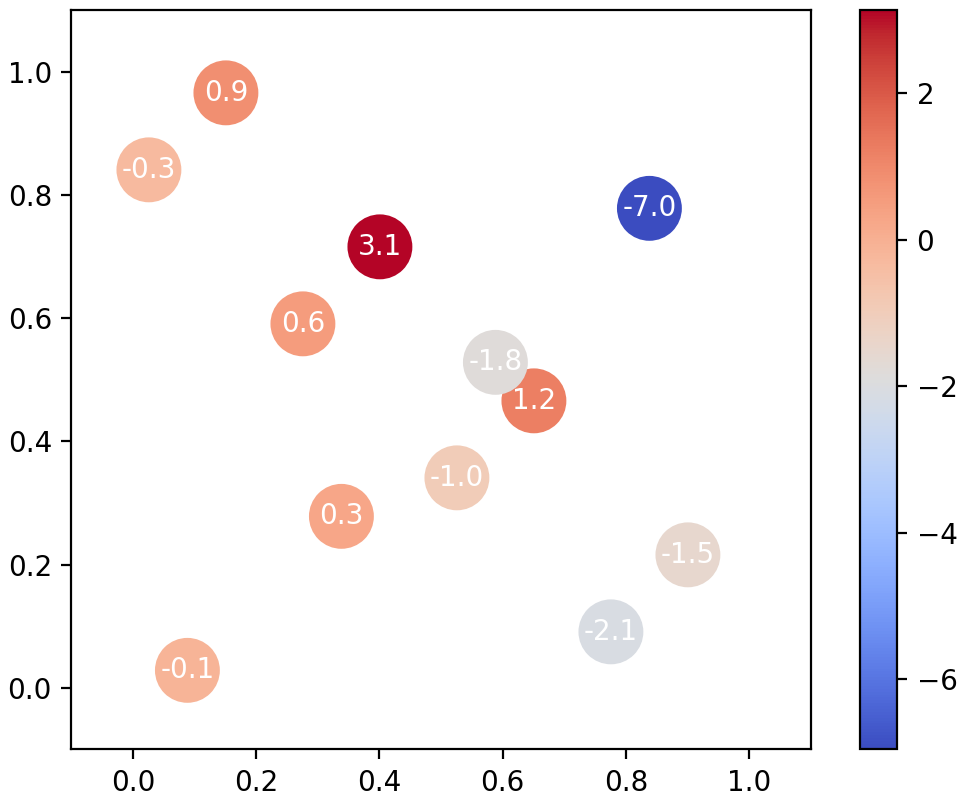
\includegraphics[width=\textwidth]{assets/1d-sobol-1st}
		\caption{}
	\end{subfigure}
	\begin{subfigure}[b]{0.325\textwidth}
		\centering
		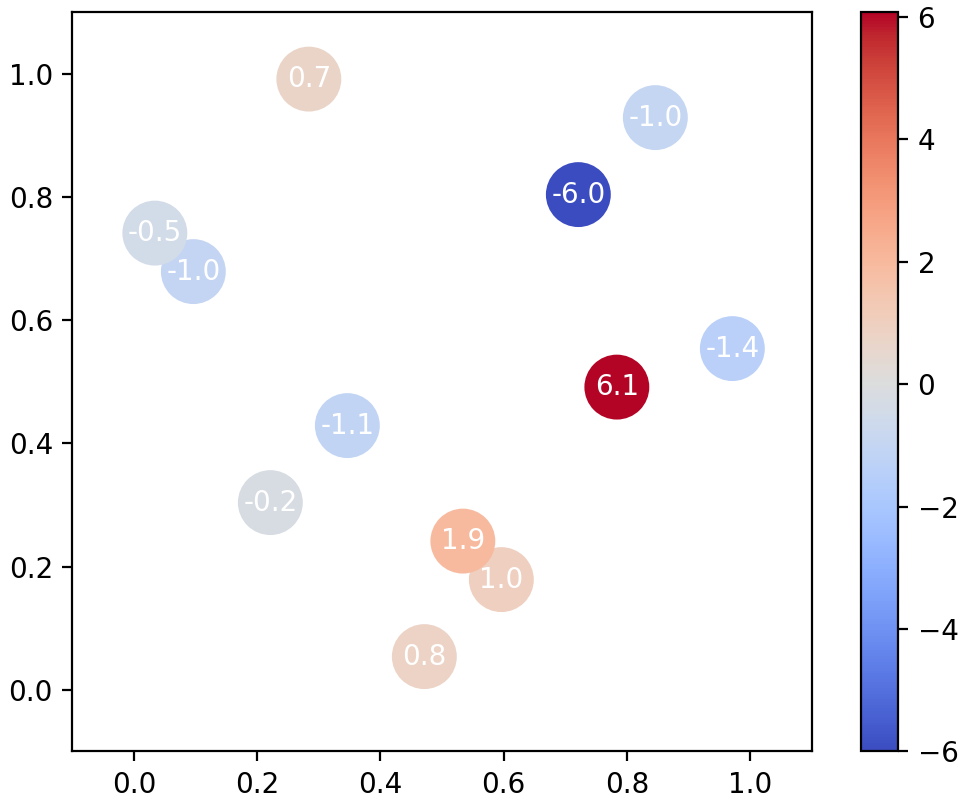
\includegraphics[width=\textwidth]{assets/1d-sobol-2nd}
		\caption{}
	\end{subfigure}
	\begin{subfigure}[b]{0.325\textwidth}
		\centering
		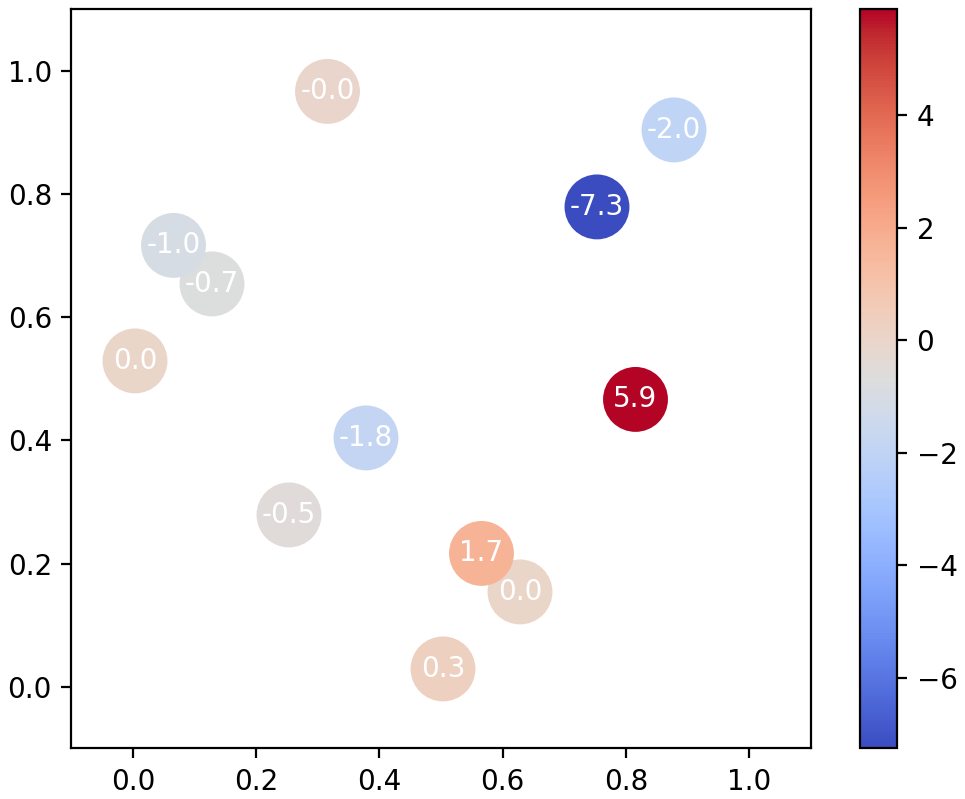
\includegraphics[width=\textwidth]{assets/1d-sobol-3rd}
		\caption{}
	\end{subfigure}

	\caption{Results of three random search trials using Sobol sequences for the hyperparameters for $f_1$ shown in (a), (b), and (c).}
	\label{fig:1d-sobol-random}
\end{figure}


\subsection{e)}\label{subsec:basic-e}

We can treat the good fraction of the HP configuration space as a probability. That is, in each trial we have the probability $p$ of picking a good configuration/being the good area of the HP configuration space. Given that we perform $n$ trials, the probability $x$ of finding at least one good HP configuration is the counterprobability of finding no good HP configuration:

\begin{equation}
	x \leq 1-(1-p)^n
\end{equation}

\noindent We can solve this by replacing the inequality with an equality:

\begin{equation}
	x = 1-(1-p)^n
\end{equation}

\begin{equation}
	(1-p)^n = 1-x
\end{equation}

\begin{equation}
	n\log(1-p) = \log(1-x)
\end{equation}

\begin{equation}
	n = \frac{\log(1-x)}{\log(1-p)}  
\end{equation}

\noindent That is, the number of trials depends on both the probability $x$ which we are trying to achieve and $p$, the good fraction of the HP space. When we have $L$ hyperparameters, the probability of finding a good HP configuration is the probability of all hyperparameters being in the good fraction of their configuration space at the same time $p^L$: 

\begin{equation}
	x = 1-(1-p^L)^n
\end{equation}

\begin{equation}
	n = \frac{\log(1-x)}{\log(1-p^L)}  
\end{equation}


\noindent That is, the number of trials necessary to find at least good HP configuration grows quasi exponentially in the number of hyperparameters $L$. This is akin to the curse of dimensionality. That is, our problem gets exponentially harder to solve as we increase the dimensionality.\\


\noindent When using grid search, we only explore $n^{1/L}$ configurations per parameter (vs. $n$ in Random Search). That is, we explore fewer configurations for the same amount of trials and will therefore need a higher number of trials to find at least one good HP configuration with a high probability $x$:

\begin{equation}
  n^{1/L}=\frac{\log(1-x)}{\log(1-p^L)}
\end{equation}

\begin{equation}
  n=\left(\frac{\log(1-x)}{\log(1-p^L)}\right)^L
\end{equation}

\noindent So, in grid search, the number of trials needed grows exponentially in the number of hyperparameters. However, we assumed that the good fraction of the HP space is interpretable as a probability. This is intuitive when using uniform random sampling. In grid search however, we do not perform random sampling but split our grid into equidistant points or use some other kind heuristic to predefine a set of values per hyperparameter to explore. Thus, the interpretation of $p$ as a probability does not work out necessarily.

\section{Gaussian Process Regression}\label{sec:gpr}

\subsection{a)}\label{subsec:gpr-a}

\autoref{fig:2a-rbf-s-ls} shows the provided scaled RBF kernel for multiple values of the \textit{scale} and \textit{length-scale} parameters. Intuitively, the \textit{length-scale} parameter controls what values are seen as similar and what values are not. For example, when inspecting the kernel with $scale=1$ and $length-scale=3$ (i.e. the solid green line), we can see that kernel assigns much higher values for a distance of $2.5$ between inputs (roughly $0.7$), whereas another kernel with $length-scale=1$ (i.e. the solid orange line) assigns a value of almost $0$ for samples that have the same distance between them. 

\begin{figure}[H]
  	\center
  	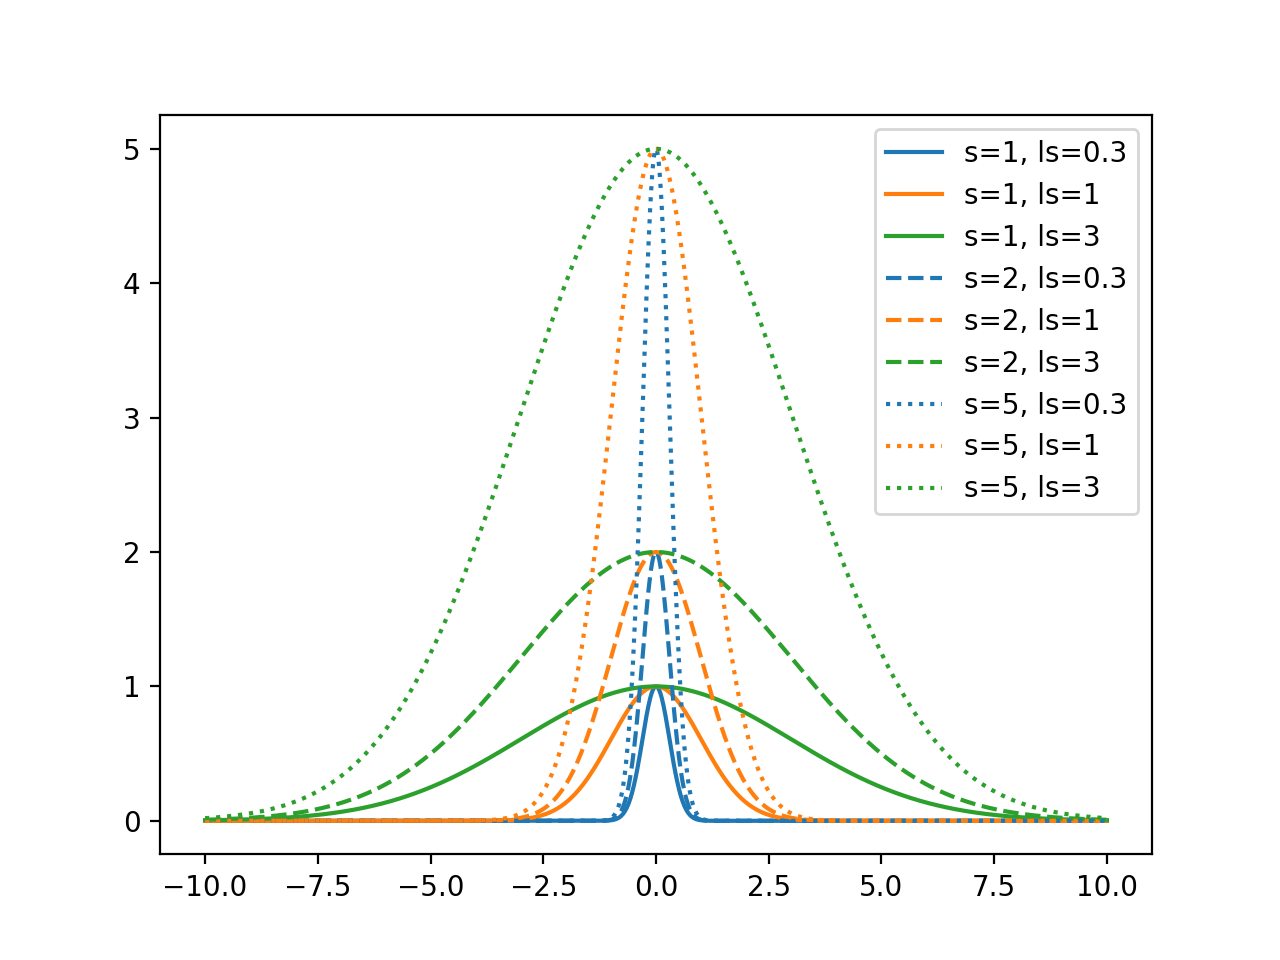
\includegraphics[width=.5\columnwidth]{assets/2a-rbf-s-ls}
  	\caption{Scaled RBF kernel for different values of the \textit{scale} and \textit{length-scale} paramters. The x-axis displays the distance between two samples and the y-axis the assigned similarity values by the kernel.}
  	\label{fig:2a-rbf-s-ls}
\end{figure}


\noindent The \textit{scale} parameter scales the similarity scores assigned to two samples by the kernel. In \autoref{fig:2a-rbf-s-ls}, we can see that when we keep the \textit{length-scale} parameter fixed and vary the \textit{scale}, the similarity values for the same distances between samples are either scaled up or down.

The used kernel function is a scaled RBF kernel. The RBF kernel is multiplied with the constant kernel, whose value is controlled by the \textit{scale} parameter:

\begin{gather*}
  \kappa_{scaled-RBF}(\mathbf{x_1},\mathbf{x_2})=const * \exp\left(\frac{\lVert \mathbf{x_1} - \mathbf{x_1} \rVert^2}{2\sigma^2}\right) \\
	\text{where $const = scale$ and $\sigma=length-scale$}
	\label{eq:scaled-rbf-kernel}
\end{gather*}

\subsection{b)}\label{subsec:gpr-b}

As discussed in the previous subsection (cf. \autoref{subsec:gpr-a}), the \textit{scale} parameter scales the outputs of the kernel whereas the \textit{length-scale} parameter controls which values are seen as similar by the kernel. Now, when we sample from a GP prior we can see the effect of these parameters in \autoref{fig:2b-srbf-kernels}. We vary the \textit{scale} by column and the \textit{length-scale} by row. We can observe that smaller length scale values correspond to "noisier" functions (i.e. the function values vary more). Higher \textit{scale} values just scale the y-axis up or down. So, we can say that we sample smoother functions for larger \textit{length-scales} and vice-versa for smaller values.

\begin{figure}[H]
  	\center
  	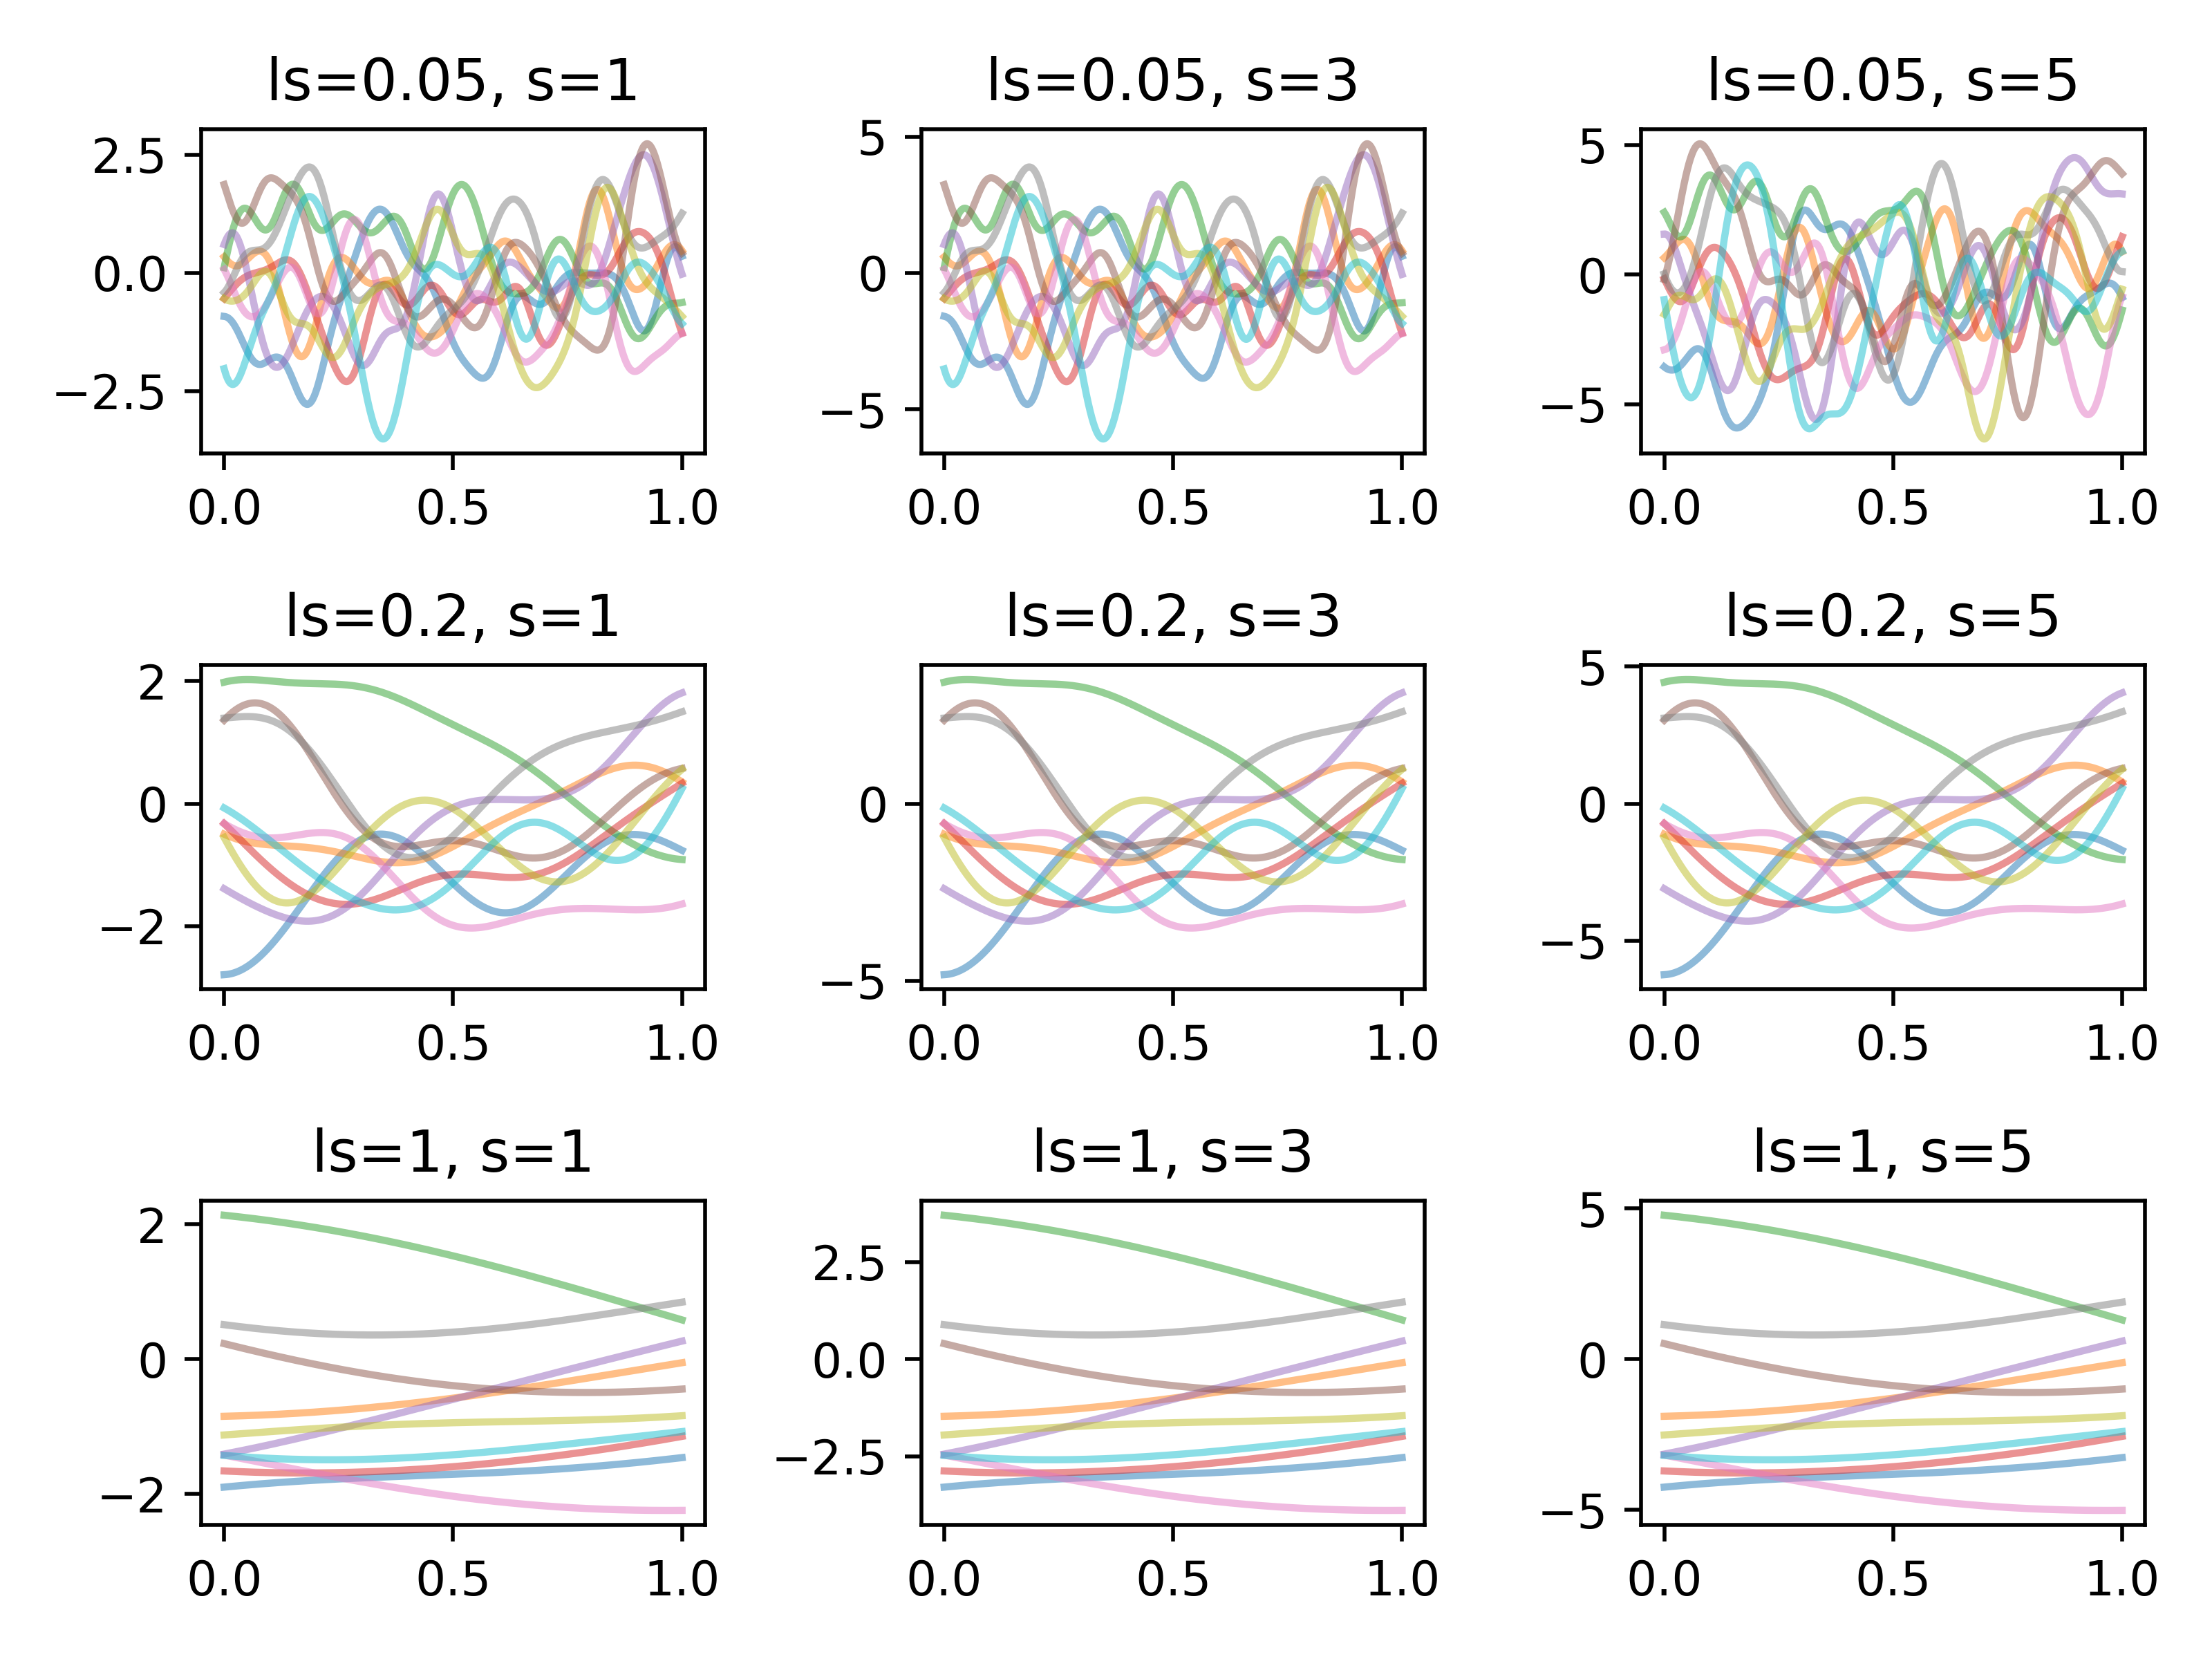
\includegraphics[width=\columnwidth]{assets/2b-srbf-kernels}
  	\caption{Samples from a Gaussian Process priors using the provided sclaed RBF kernel with different \textit{length-scale} and \textit{scale} parameters.}
  	\label{fig:2b-srbf-kernels}
\end{figure}

\subsection{c)}\label{subsec:gpr-c}

\autoref{fig:2c-f2} shows the plot for function $f_2$. We can see that the minimum of the function is to the right of our observation at $x=0.5$. With three observations, we evaluate the function at $x\in \{0, 0.5, 1\}$. However, we can see that the (global) minimum is to the right of our observation at $x=0.5$ and that the function values have a lot higher variance in the right side of the input domain. Also, with only three observations, we will not be able to approximate $f_2$ very well with Gaussian Process Regression. Hence, we will need to use a prior that encodes a high uncertainty such that we are also likely to find our global minimum. Therefore, we used a very low \textit{length-scale} of $0.03$ and a \textit{scale} of $0.36$. 

\begin{figure}[H]
  	\center
  	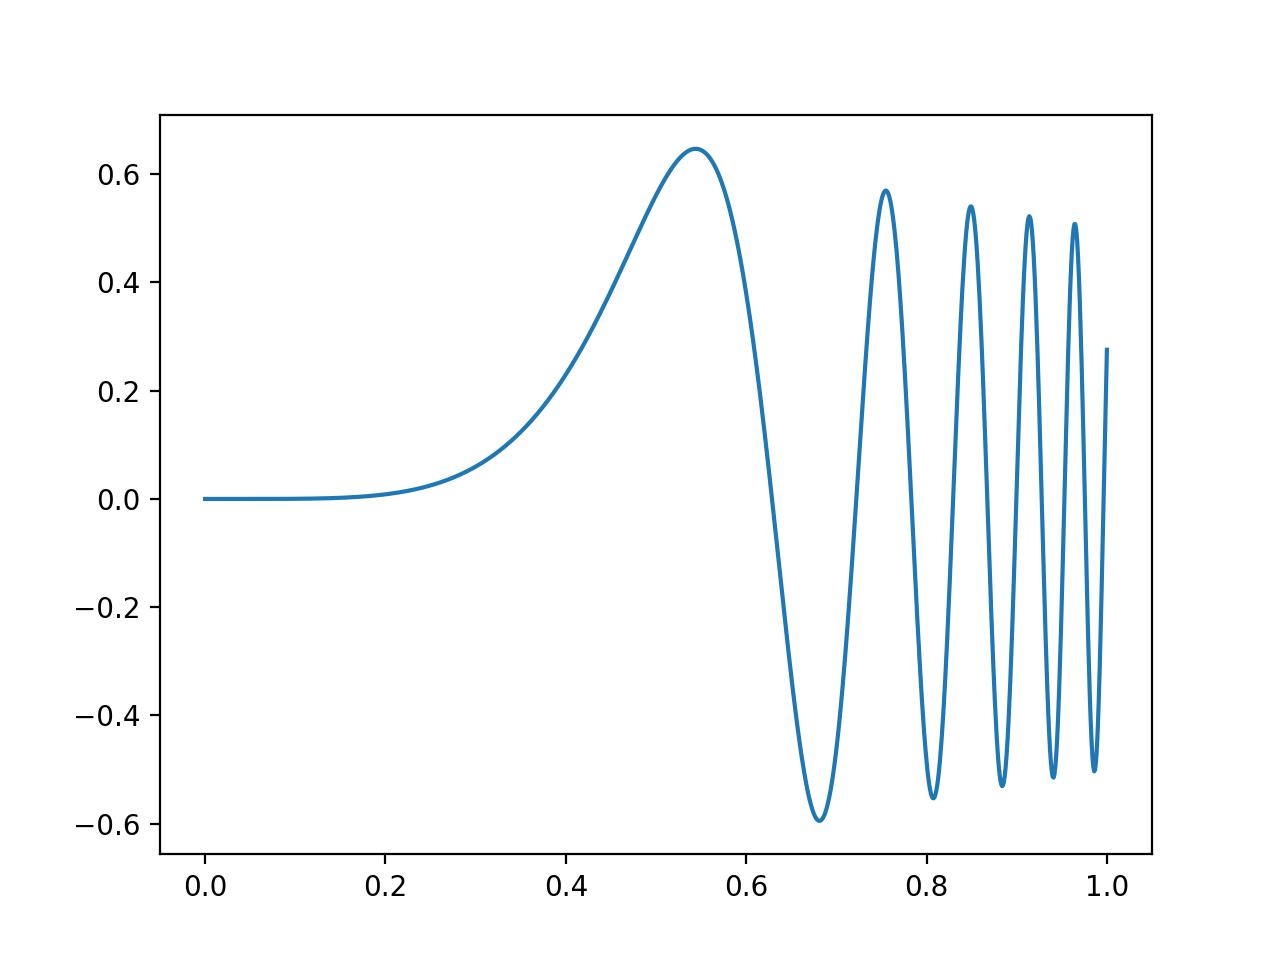
\includegraphics[width=.5\columnwidth]{assets/2c-f2}
  	\caption{Plot showing $f_2$}
  	\label{fig:2c-f2}
\end{figure}

\noindent As expected, we cannot approximate the function well with only three observations. Our posterior mean does not capture any of the variance in $f_2$ in the right side of the input domain and misses our global minimum completly. The posterior variance is low for values (very) close to our observations, but quickly increases for values that are further away as can be seen by the orange bounds in \autoref{fig:2c-posterior}. 

\begin{figure}[H]
  	\center
  	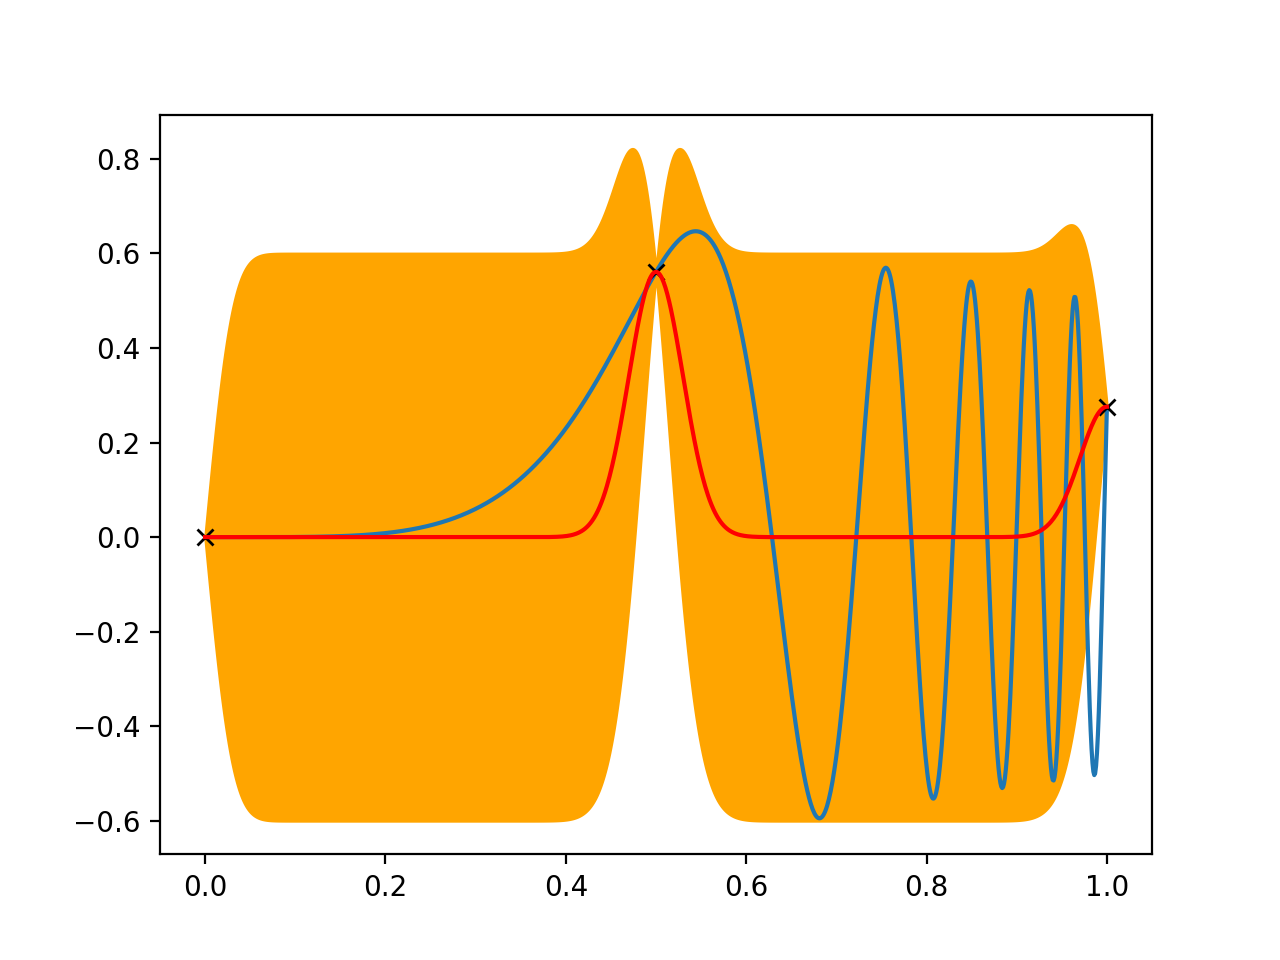
\includegraphics[width=.5\columnwidth]{assets/2c-posterior}
  	\caption{Posterior of the Gaussian Process Regression for $f_2$ with $s=0.36$ and $ls=0.03$.}
  	\label{fig:2c-posterior}
\end{figure}

\noindent We can also see that our global optimum lies within the region of uncertainty (posterior variance). Therefore, we are likely to evaluate $f_2$ at input values close to the global optimum during bayesian optimization. We can therefore conjecture that we are likely to converge to the global optimum and that are our kernel parameters were chosen properly given that we only have three observations. However, if we had more oberservations we could use a prior that encodes a lower uncertainty and likely need less trials to find the global optimum. 


\subsection{d)}\label{subsec:gpr-d}

In \autoref{fig:2d} we varied the number of samples ($n\in\{6,12,18\}$) by column and the \textit{length-scale} ($ls\in\{0.03, 0.045, 0.0675\}$) while keeping the \textit{scale} fixed at $0.36$. 

\begin{figure}[H]
  	\center
  	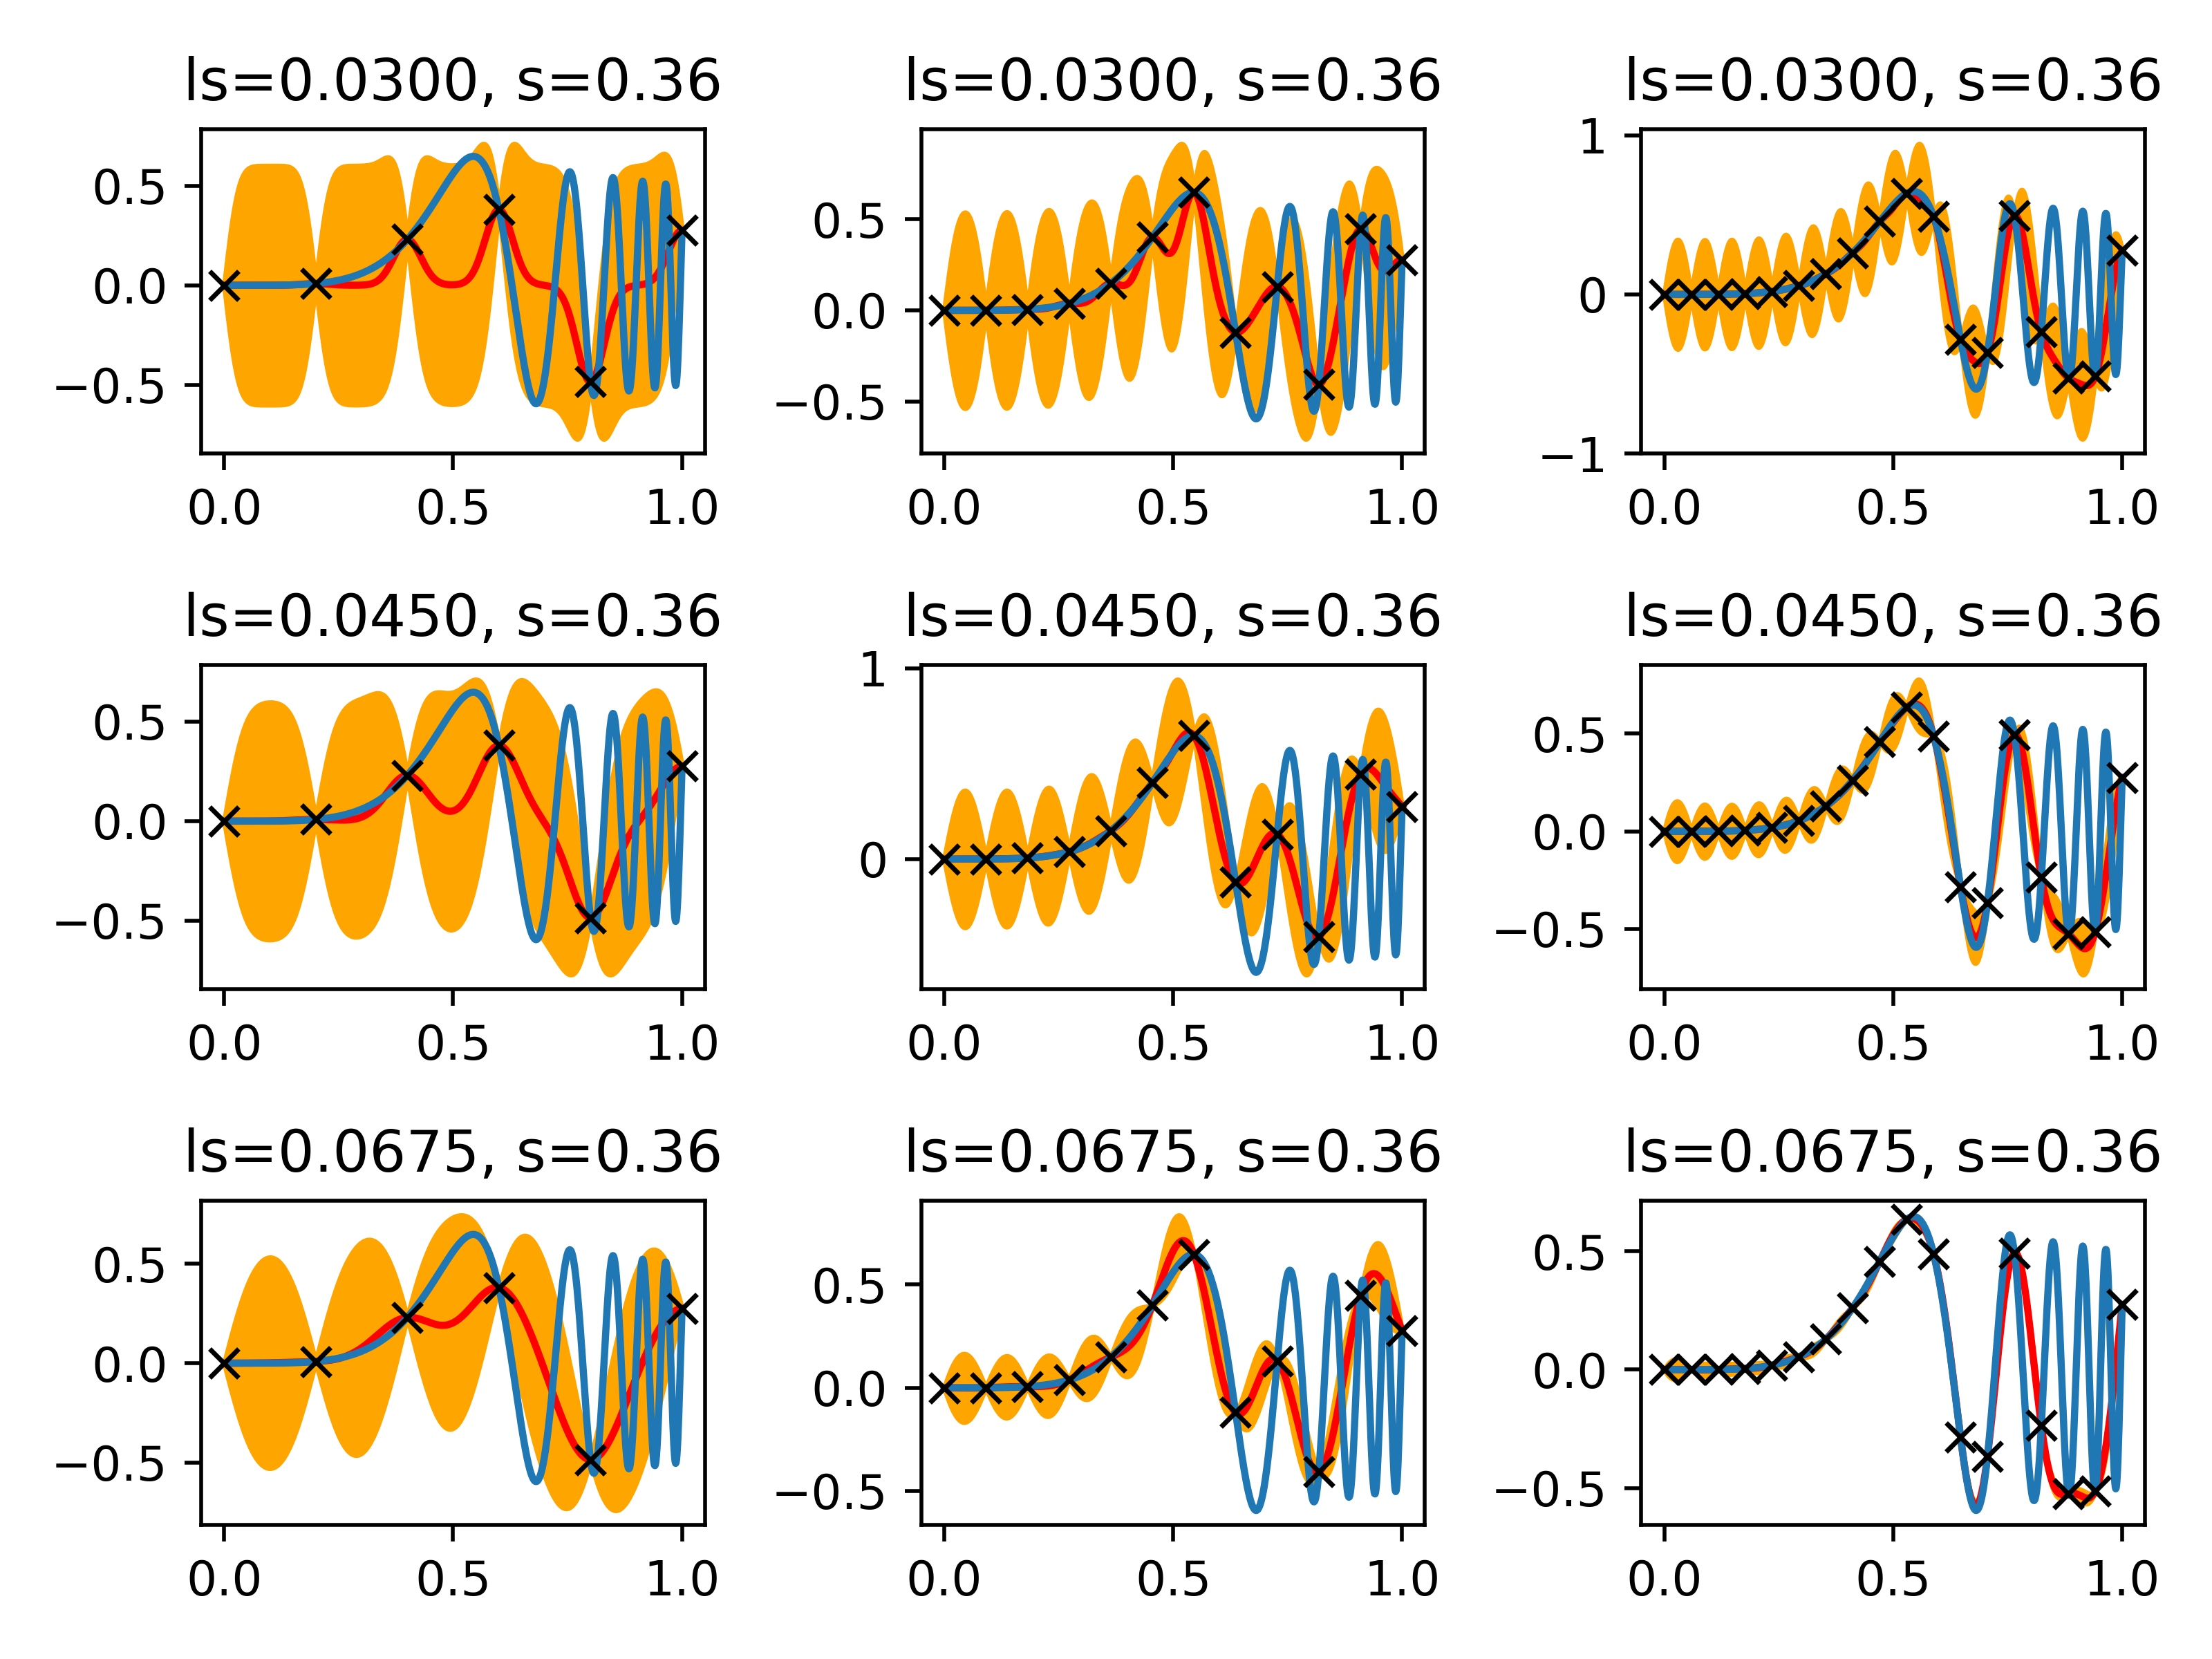
\includegraphics[width=\textwidth]{assets/2d}
  	\caption{Varying the number of samples (by column: 6, 12, 18) and the magnitude of the \textit{length-scale} parameter (multiplied by 1.5 in each row, starting with 0.03).}
  	\label{fig:2d}
\end{figure}

\noindent We can observe that our approximation of the underlying function $f_2$ improves as we increase the number of samples, which is to be expected. We can also observe that increasing the \textit{length-scale} does not necessarily improve our fit to the function. In fact, increasing the length-scale does nothing to capture the variability of function values in the right side of the input domain, as discussed previously. With $n=18$ observations and $ls=0.0675$, we fit the function quite well and would find the global optimum with bayesian optimization. We can also see that we underfit $f_2$ everywhere, though this does not prevent us from finding the global minimum. That is, for all cases with $n=18$, we would likely find the global optimum as visible in the figure above. Also, it is entirely possible that our prior is not suitable for the functional form of $f_2$ and that we may want to consider a combination of multiple kernels (i.e. perhaps two: one for the right side of the domain, and one for the left).

\subsection{e)}\label{subsec:gpr-e}

If we were to use bayesian optimization with our prior from \autoref{fig:2c-posterior} and three observations, it would not be guaranteed that we find the global minimum. In fact, it would be very likely that the model would converge in one of the (four) local minimima (cf. \autoref{fig:2c-f2}). This is because our prior is quite uninformative for large regions of the input domain (i.e. everything that is not in the direct vicinity of the given observations). That is, we would likely start sampling randomly in areas where the uncertainty is at it's maximum (most of the input domain). 

\section{Bayesian Optimization}\label{sec:bayes_opt}

\autoref{fig:3-f1-f2} shows the results of bayesian optimization for $f_1$ and $f_2$. To run bayesian optimization, the package BayesianOptimization \cite{nogueira2014bayes} was used with standard settings (prior observations = 3; number of iterations = 30). We, again, used three prior observations as our history and then ran 30 trials of bayesian optimization for both functions. Both optimizers converged to the global minimum (or got very close): $\hat{y}=-7.886$ and $[0.792, 0.7916 ]$ for $f_1$, and $\hat{y}=-0.5947$ and $[0.6812]$ for $f_2$. Note that we had to rewrite the functions: since the package is only meant to find the maximum of a given function we wrote wrapper functions that return the negative function values. Hence, the plot in \autoref{fig:3-f1-f2} (b) shows an inverted version of $f_2$. We can see the difference between exploration and exploitation in the \autoref{fig:3-f1-f2} (a) where in the beginning many different HP configurations are tested our and then after $\sim$ 25 evaluations, our model switches to exploitation.


\begin{figure}[H]
	\centering
	\begin{subfigure}[b]{.35\textwidth}
		\centering
		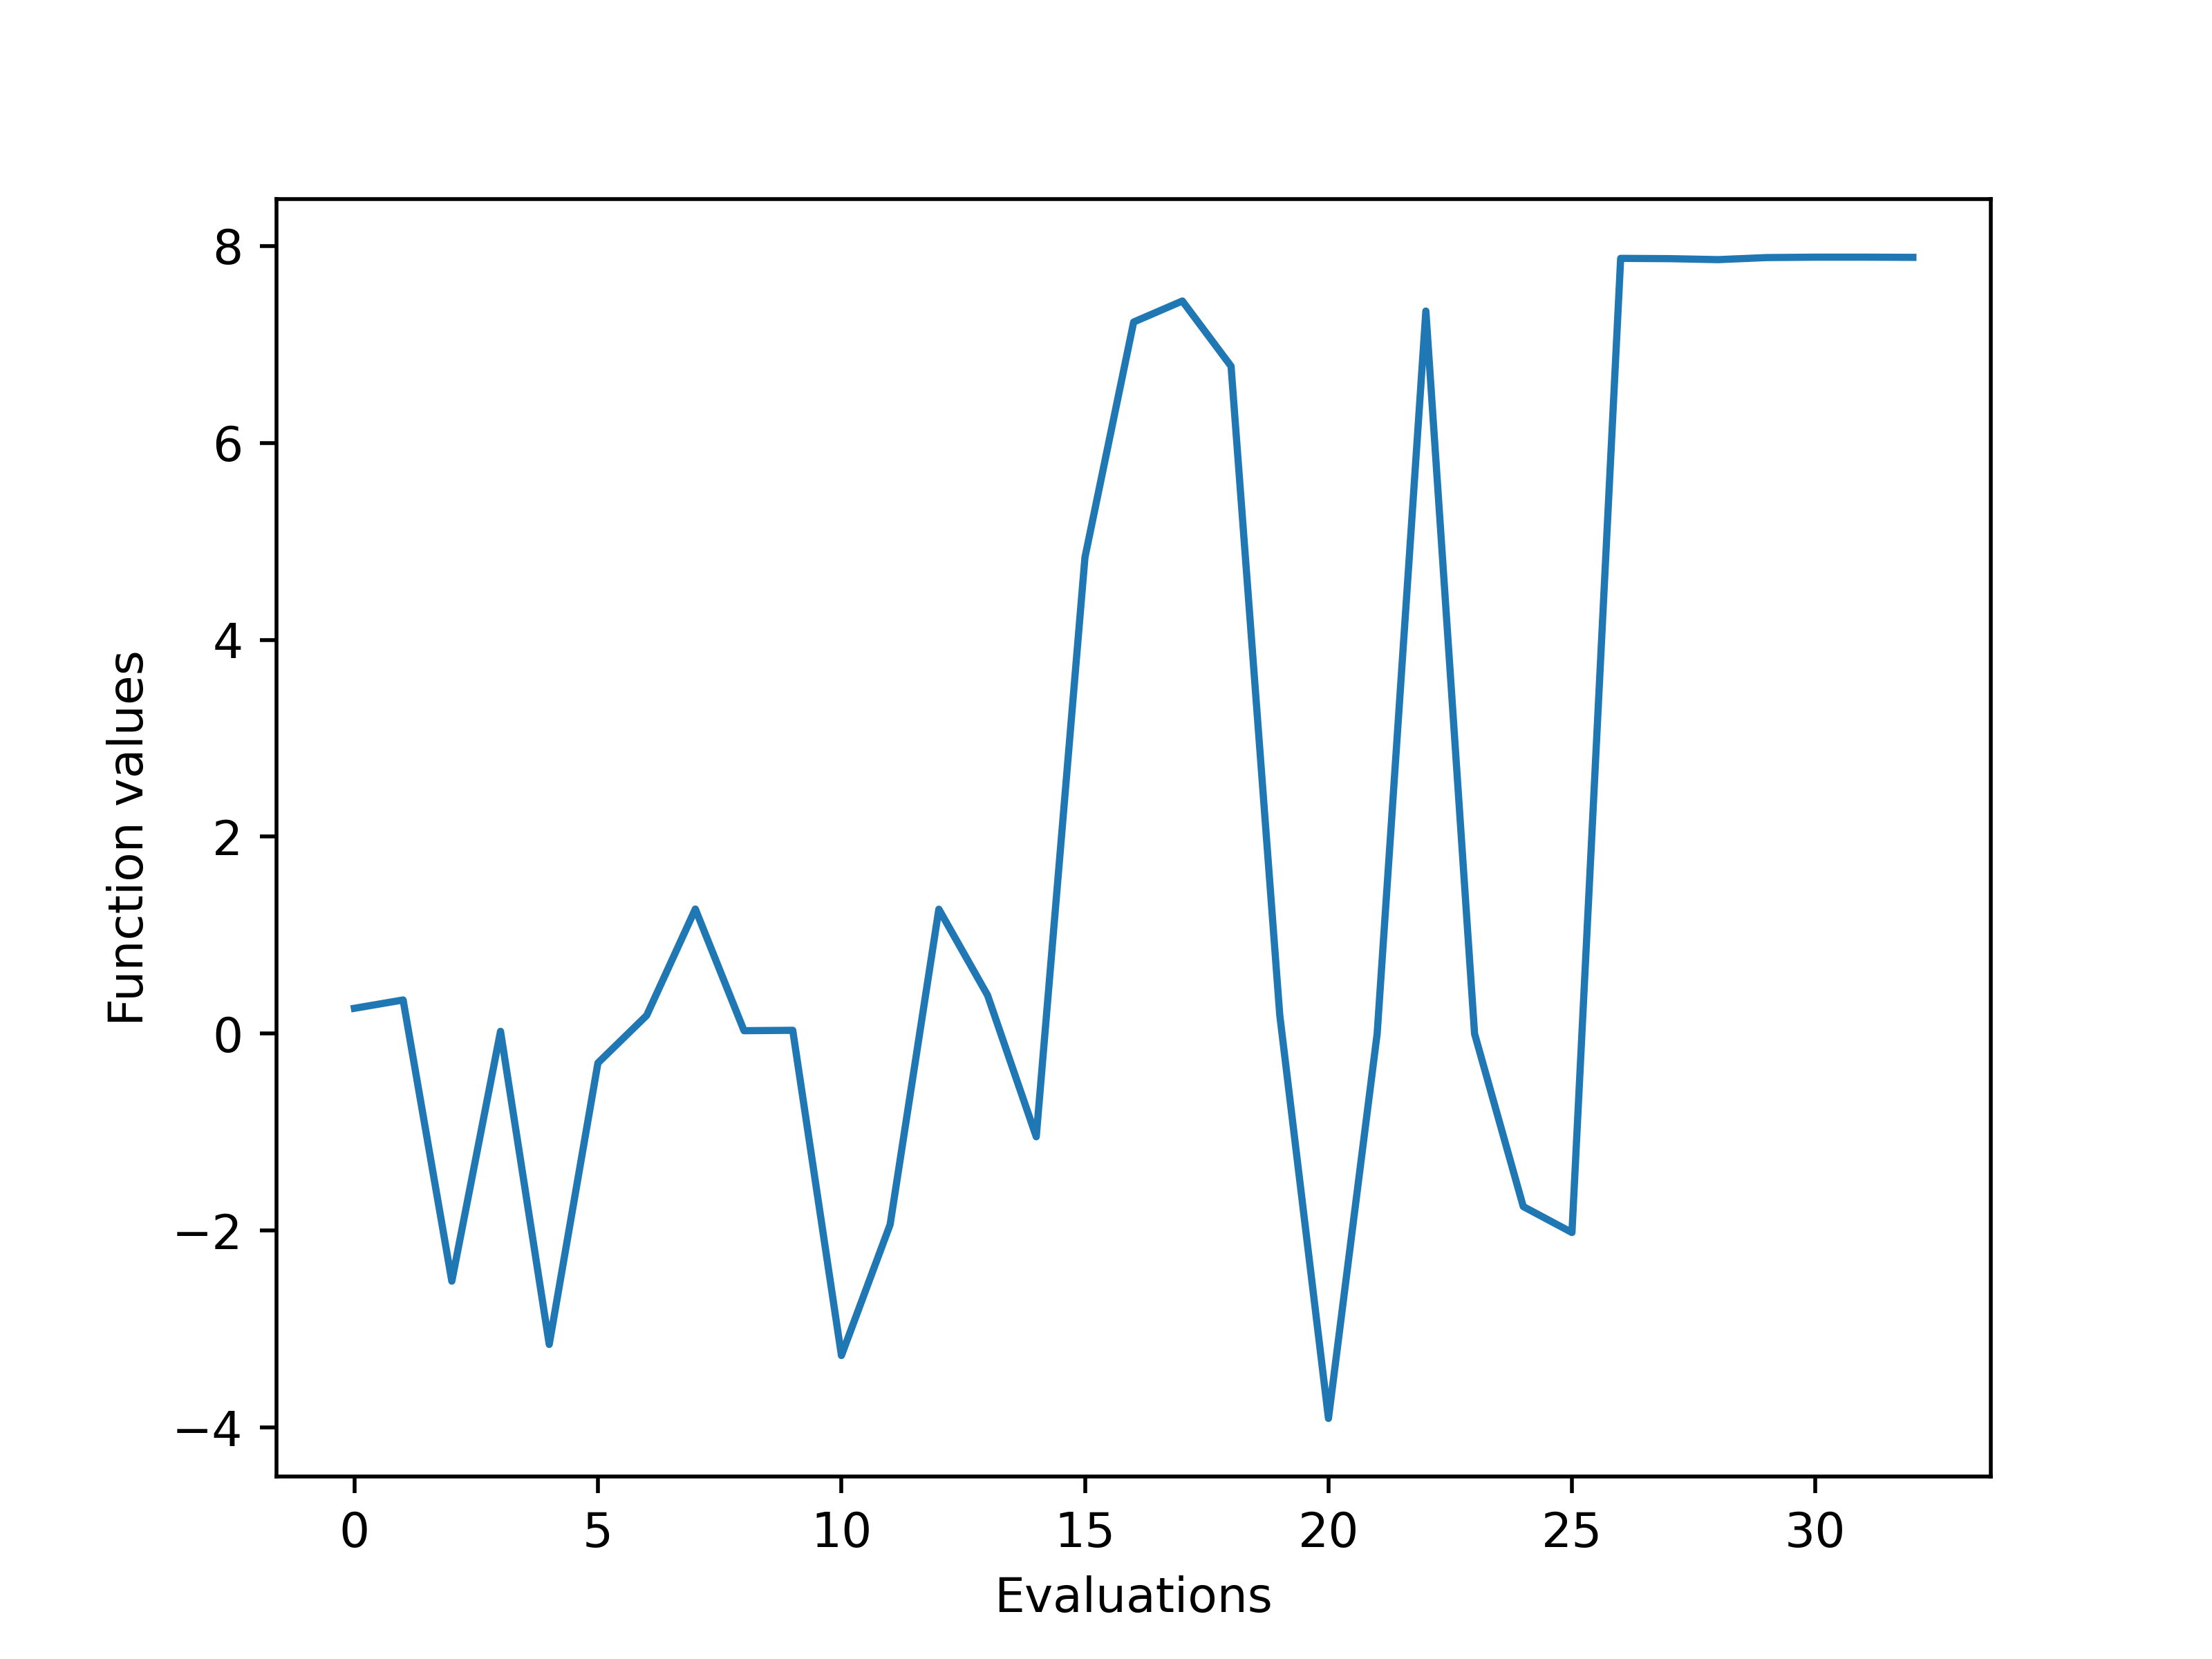
\includegraphics[width=\textwidth]{assets/3-f1}
		\caption{}
	\end{subfigure}
	\begin{subfigure}[b]{.35\textwidth}
		\centering
		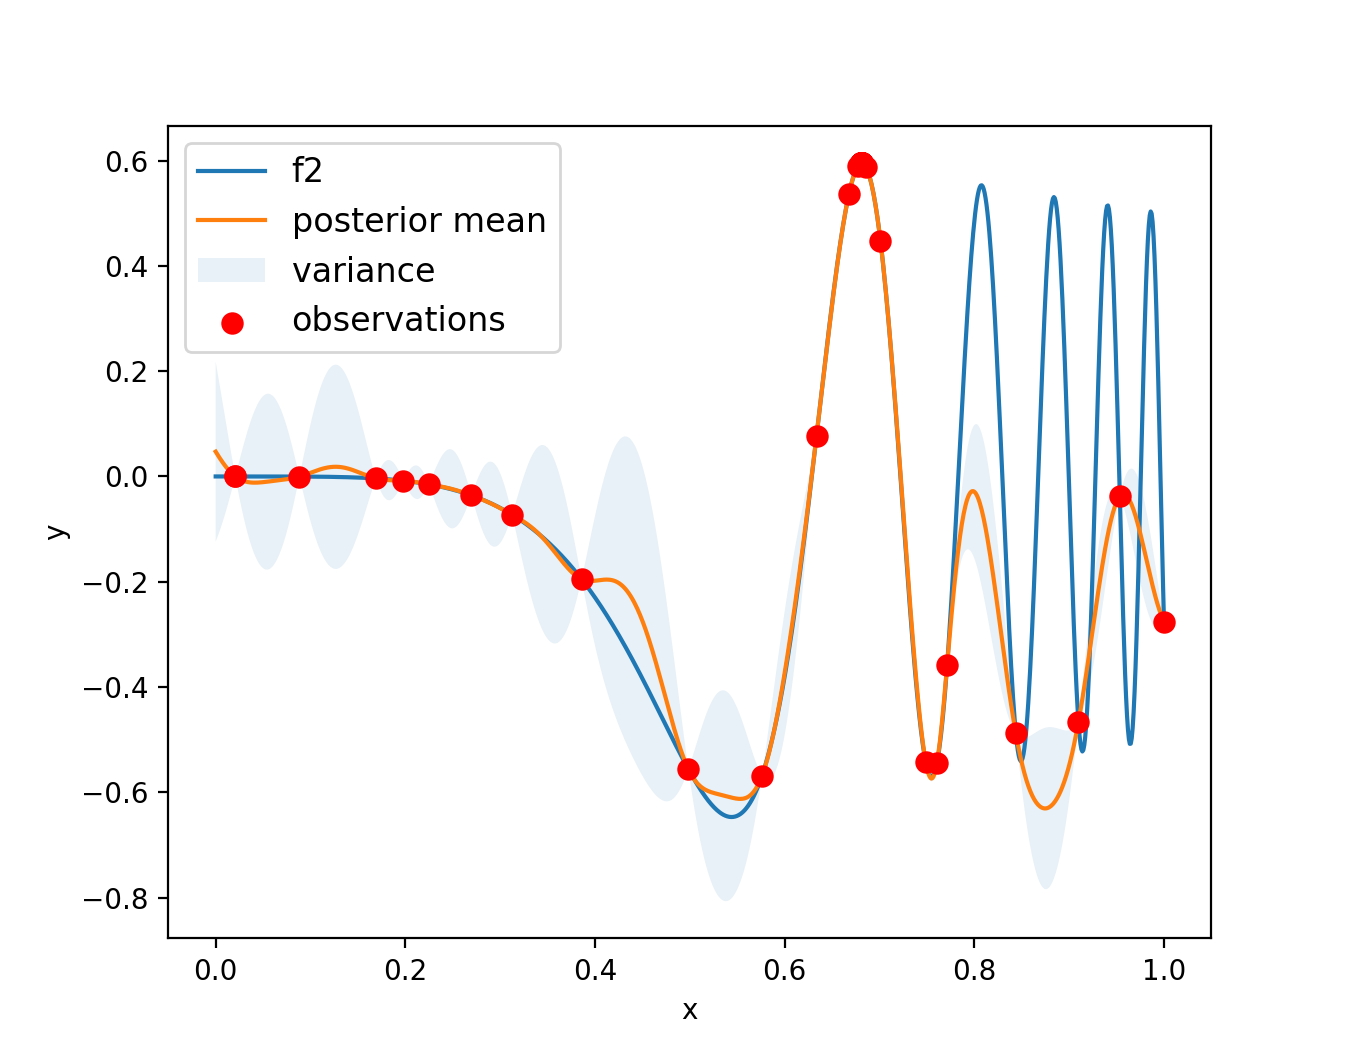
\includegraphics[width=\textwidth]{assets/3-f2}
		\caption{}
	\end{subfigure}

	\caption{Results of runnning bayesian optimization for $f_1$ and $f_2$: (a) shows the evaluated function values for $f_1$; (b) shows $f_2$, the posterior mean and variance and the observations of function values that were evaluated during bayesian optimization.}
	\label{fig:3-f1-f2}
\end{figure}


\bibliographystyle{alpha}
\bibliography{references}

\end{document}
